\documentclass{article}
\usepackage{enumerate}
\usepackage{amsmath}
\usepackage{amssymb}
\usepackage{graphicx}
\usepackage{subfigure}
\usepackage{geometry}
\usepackage{caption}
\usepackage{indentfirst}
\usepackage{tikz}
\usetikzlibrary{circuits.logic.US}
\usetikzlibrary{arrows.meta}
\usetikzlibrary{calc}
\geometry{left=3.0cm,right=3.0cm,top=3.0cm,bottom=3.0cm}
\renewcommand{\thesection}{Problem \arabic{section}.}
\title{VE270 Homework 7}
\author{Liu Yihao 515370910207}
\date{}

\begin{document}
\maketitle

\section{}
\begin{center}
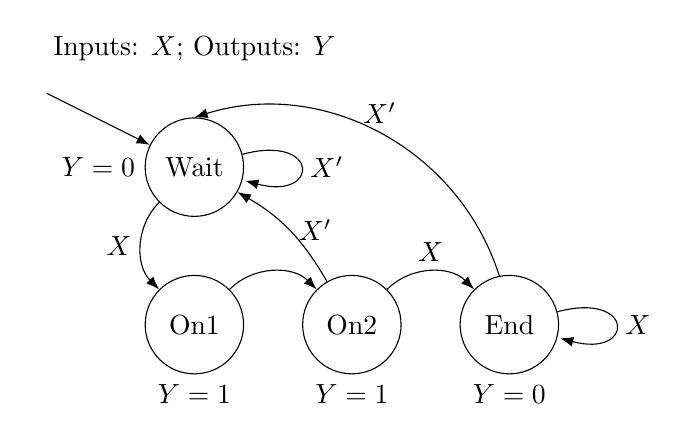
\begin{tikzpicture}[>/.tip={Latex}]
	\draw (0,0.5) node (io) {Inputs: $X$; Outputs: $Y$};
	\draw (0,-1) node (wait) [draw,shape=circle,minimum size=1.25cm] {Wait};
	\node [left] at (wait.west) {$Y=0$};
	\draw (0,-3) node (on1) [draw,shape=circle,minimum size=1.25cm] {On1};
	\node [below] at (on1.south) {$Y=1$};
	\draw (2,-3) node (on2) [draw,shape=circle,minimum size=1.25cm] {On2};
	\node [below] at (on2.south) {$Y=1$};
	\draw (4,-3) node (end) [draw,shape=circle,minimum size=1.25cm] {End};
	\node [below] at (end.south) {$Y=0$};

	\draw[->] (wait) edge [loop right] node {$X'$} ();
	\draw[->] (wait) edge [bend right=45] node [left] {$X$} (on1);
	\draw[->] (on1) edge [bend left=45] node {} (on2);
	\draw[->] (on2) edge [bend left=45] node [above] {$X$} (end);
	\draw[->] (on2) [bend right=15] edge node [right] {$X'$} (wait);
	\draw[->] (end) edge [loop right] node {$X$} ();
	\draw[->] (end) edge [bend right=45] node [above] {$X'$} (wait.north);
	
	\draw (-2,0) node (init) {};
	\draw[->] (init) edge (wait);
\end{tikzpicture}
\end{center}

\section{}
Encode the states ($s_1s_0$): Wait: 00, On1: 10, On2: 11, End: 01. \\

The truth table is 

\begin{center}
\begin{tabular}{ccc|ccc}
$s_{1}$ & $s_{0}$ & $X$ & $n_{1}$ & $n_{0}$ & $Y$ \\
\hline
0 & 0 & 0 & 0 & 0 & 0 \\
0 & 0 & 1 & 1 & 0 & 0 \\
0 & 1 & 0 & 0 & 0 & 0 \\
0 & 1 & 1 & 0 & 1 & 0 \\
1 & 0 & 0 & 1 & 1 & 1 \\
1 & 0 & 1 & 1 & 1 & 1 \\
1 & 1 & 0 & 0 & 0 & 1 \\
1 & 1 & 1 & 0 & 1 & 1 \\
\end{tabular}
\end{center}

The euqations are 

$$n_{1}=s_{0}'X+s_{1}s_{0}'$$
$$n_{0}=s_{0}X+s_{1}s_{0}'$$
$$Y=s_{1}$$


The schematics is 

\begin{center}
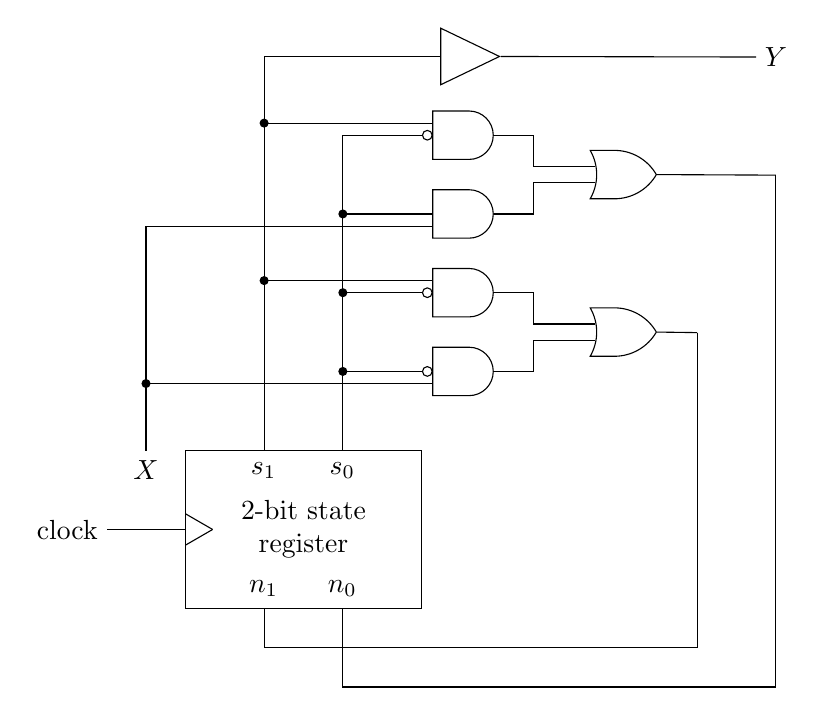
\begin{tikzpicture}[circuit logic US]
\draw (0,0) node (r) [shape=rectangle,draw,minimum height=2cm,minimum width=3cm,text width=2cm,align=center] {2-bit state register};
\draw (-3,0) node (clock) {clock};\draw (clock) -- (r.west);\draw (r) ++(left:11.54mm) -- ++($(left:3.46mm)+(down:2mm)$);
\draw (r) ++(left:11.54mm) -- ++($(left:3.46mm)+(up:2mm)$);
\draw (r.west) ++(up:7.5mm) ++(right:10.000000mm) node {$s_1$};
\draw (r.west) ++(down:7.5mm) ++(right:10.000000mm) node {$n_1$};
\draw (r.west) ++(up:7.5mm) ++(right:20.000000mm) node {$s_0$};
\draw (r.west) ++(down:7.5mm) ++(right:20.000000mm) node {$n_0$};
\draw (-2.000000,0.750000) node {$X$};
\draw (r.north) ++(up:1.000000cm) ++(right:2cm) node (and1) [and gate,inputs=nin] {};
\draw (0.500000,1.000000) |- (and1.input 2) ;
\draw (-2.000000,1.000000) |- (and1.input 3) ;
\draw (r.north) ++(up:2.000000cm) ++(right:2cm) node (and2) [and gate,inputs=nin] {};
\draw (-0.500000,1.000000) |- (and2.input 1) ;
\draw (0.500000,1.000000) |- (and2.input 2) ;
\draw (and1.input 2) ;
\pgfgetlastxy{\x}{\y};
\filldraw (0.500000,\y) circle [radius=0.5mm];
\draw (r.north) ++(up:1.500000cm) ++(right:4cm) node (or1) [or gate,inputs=nn] {};
\draw (and1.output) -- ++(right:0.500000cm) |- (or1.input 2);
\draw (and2.output) -- ++(right:0.500000cm) |- (or1.input 1);
\draw (or1.output) -- (5.000000,2.500000);
\draw (5.000000,2.500000) -- (5.000000,-1.500000) -| (-0.500000,-1);
\draw (r.north) ++(up:3.000000cm) ++(right:2cm) node (and3) [and gate,inputs=nnn] {};
\draw (0.500000,1.000000) |- (and3.input 2) ;
\draw (-2.000000,1.000000) |- (and3.input 3) ;
\draw (and2.input 2) ;
\pgfgetlastxy{\x}{\y};
\filldraw (0.500000,\y) circle [radius=0.5mm];
\draw (and1.input 3) ;
\pgfgetlastxy{\x}{\y};
\filldraw (-2.000000,\y) circle [radius=0.5mm];
\draw (r.north) ++(up:4.000000cm) ++(right:2cm) node (and4) [and gate,inputs=nin] {};
\draw (-0.500000,1.000000) |- (and4.input 1) ;
\draw (0.500000,1.000000) |- (and4.input 2) ;
\draw (and2.input 1) ;
\pgfgetlastxy{\x}{\y};
\filldraw (-0.500000,\y) circle [radius=0.5mm];
\draw (and3.input 2) ;
\pgfgetlastxy{\x}{\y};
\filldraw (0.500000,\y) circle [radius=0.5mm];
\draw (r.north) ++(up:3.500000cm) ++(right:4cm) node (or2) [or gate,inputs=nn] {};
\draw (and3.output) -- ++(right:0.500000cm) |- (or2.input 2);
\draw (and4.output) -- ++(right:0.500000cm) |- (or2.input 1);
\draw (or2.output) -- (6.000000,4.500000);
\draw (6.000000,4.500000) -- (6.000000,-2.000000) -| (0.500000,-1);
\draw (r.north) ++(up:5.000000cm) ++(right:2cm) node (and5) [buffer gate] {};
\draw (-0.500000,1.000000) |- (and5.input) ;
\draw (and4.input 1) ;
\pgfgetlastxy{\x}{\y};
\filldraw (-0.500000,\y) circle [radius=0.5mm];
\draw (and5.output) -- (5.750000,6.000000);
\draw (6,6.000000) node {$Y$};
\end{tikzpicture}
\end{center}


\section{}
\begin{center}
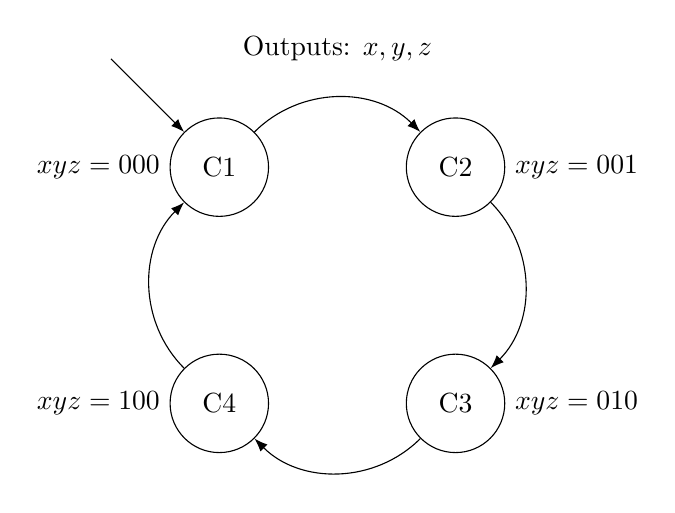
\begin{tikzpicture}[>/.tip={Latex}]
	\draw (0,3) node (io) {Outputs: $x,y,z$};
	\draw (-1.5,1.5) node(C1) [draw,shape=circle,minimum size=1.25cm] {C1};
	\node [left] at (C1.west) {$xyz=000$};
	\draw (1.5,1.5) node(C2) [draw,shape=circle,minimum size=1.25cm] {C2};
	\node [right] at (C2.east) {$xyz=001$};
	\draw (1.5,-1.5) node(C3) [draw,shape=circle,minimum size=1.25cm] {C3};
	\node [right] at (C3.east) {$xyz=010$};
	\draw (-1.5,-1.5) node(C4) [draw,shape=circle,minimum size=1.25cm] {C4};
	\node [left] at (C4.west) {$xyz=100$};
	\draw[->] (C1) edge [bend left=45] (C2);
	\draw[->] (C2) edge [bend left=45] (C3);
	\draw[->] (C3) edge [bend left=45] (C4);
	\draw[->] (C4) edge [bend left=45] (C1);
	
	\draw (-3,3) node (init) {};
	\draw[->] (init) edge (C1);
\end{tikzpicture}
\end{center}

\section{}
\begin{center}
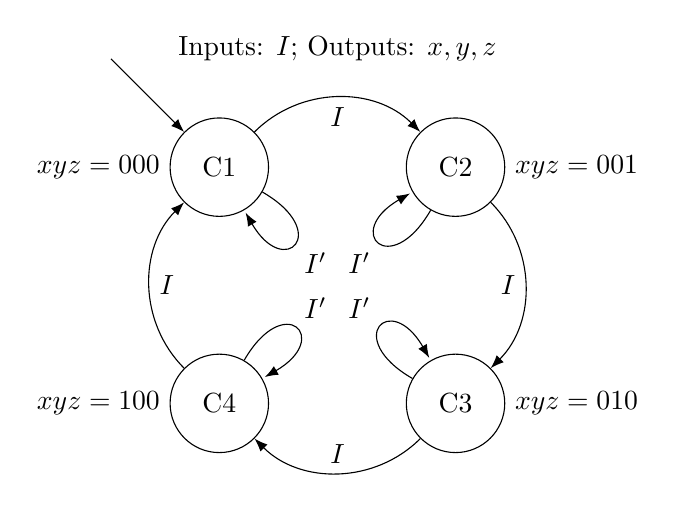
\begin{tikzpicture}[>/.tip={Latex}]
	\draw (0,3) node (io) {Inputs: $I$; Outputs: $x,y,z$};
	\draw (-1.5,1.5) node(C1) [draw,shape=circle,minimum size=1.25cm] {C1};
	\node [left] at (C1.west) {$xyz=000$};
	\draw (1.5,1.5) node(C2) [draw,shape=circle,minimum size=1.25cm] {C2};
	\node [right] at (C2.east) {$xyz=001$};
	\draw (1.5,-1.5) node(C3) [draw,shape=circle,minimum size=1.25cm] {C3};
	\node [right] at (C3.east) {$xyz=010$};
	\draw (-1.5,-1.5) node(C4) [draw,shape=circle,minimum size=1.25cm] {C4};
	\node [left] at (C4.west) {$xyz=100$};
	\draw[->] (C1) edge [bend left=45] node [below] {$I$} (C2);
	\draw[->] (C2) edge [bend left=45] node [left] {$I$} (C3);
	\draw[->] (C3) edge [bend left=45] node [above] {$I$} (C4);
	\draw[->] (C4) edge [bend left=45] node [right] {$I$} (C1);
	\draw[->] (C1) edge [in=300,out=330,loop] node [below right] {$I'$} ();
	\draw[->] (C2) edge [in=210,out=240,loop] node [below left] {$I'$} ();
	\draw[->] (C3) edge [in=120,out=150,loop] node [above left] {$I'$} ();
	\draw[->] (C4) edge [in=30,out=60,loop] node [above right] {$I'$} ();
	
	\draw (-3,3) node (init) {};
	\draw[->] (init) edge (C1);
\end{tikzpicture}
\end{center}

\section{}
\begin{center}
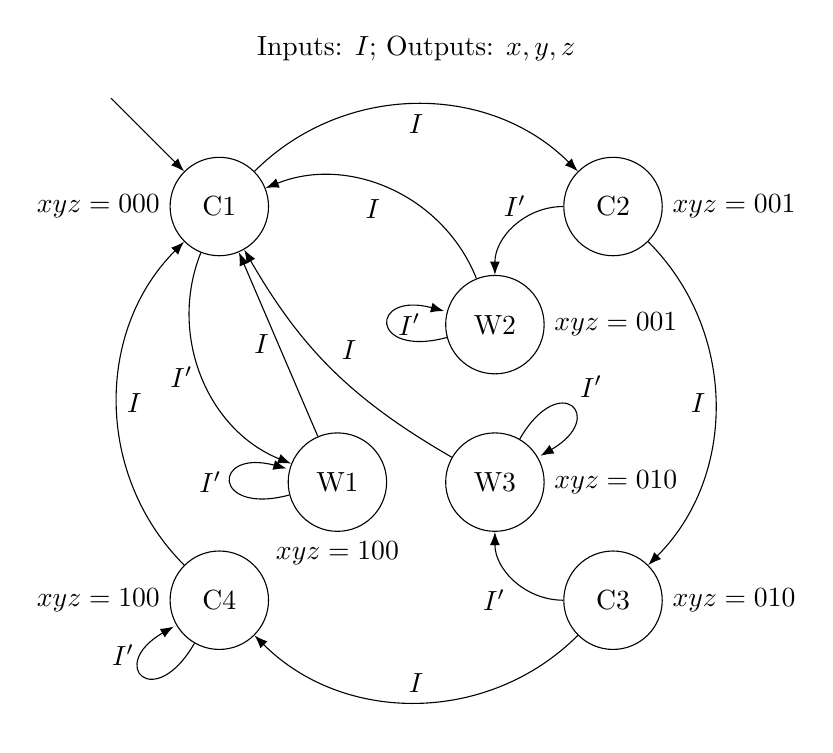
\begin{tikzpicture}[>/.tip={Latex}]
	\draw (0,4.5) node (io) {Inputs: $I$; Outputs: $x,y,z$};
	\draw (-2.5,2.5) node (C1) [draw,shape=circle,minimum size=1.25cm] {C1};
	\node [left] at (C1.west) {$xyz=000$};
	\draw (2.5,2.5) node (C2) [draw,shape=circle,minimum size=1.25cm] {C2};
	\node [right] at (C2.east) {$xyz=001$};
	\draw (1,1) node (W2) [draw,shape=circle,minimum size=1.25cm] {W2};
	\node [right] at (W2.east) {$xyz=001$};
	\draw (2.5,-2.5) node (C3) [draw,shape=circle,minimum size=1.25cm] {C3};
	\node [right] at (C3.east) {$xyz=010$};
	\draw (1,-1) node (W3) [draw,shape=circle,minimum size=1.25cm] {W3};
	\node [right] at (W3.east) {$xyz=010$};
	\draw (-2.5,-2.5) node (C4) [draw,shape=circle,minimum size=1.25cm] {C4};
	\node [left] at (C4.west) {$xyz=100$};
	\draw (-1,-1) node (W4) [draw,shape=circle,minimum size=1.25cm] {W1};
	\node [below] at (W4.south) {$xyz=100$};
	
	\draw[->] (C1) edge [bend left=45] node [below] {$I$} (C2);
	\draw[->] (C2) edge [bend left=45] node [left] {$I$} (C3);
	\draw[->] (C3) edge [bend left=45] node [above] {$I$} (C4);
	\draw[->] (C4) edge [bend left=45] node [right] {$I$} (C1);
	\draw[->] (C4) edge [in=210,out=240,loop] node [above left] {$I'$} ();
	\draw[->] (C2) edge [bend right=45] node [above] {$I'$} (W2);
	\draw[->] (W2) edge [bend right=45] node [below left] {$I$} (C1);
	\draw[->] (C3) edge [bend left=45] node [below left] {$I'$} (W3);
	\draw[->] (W3) edge [bend left=15] node [above right] {$I$} (C1);
	\draw[->] (C1) edge [bend right=45] node [left] {$I'$} (W4);
	\draw[->] (W4) edge node [left] {$I$} (C1);
	\draw[->] (W2) edge [loop left] node [right] {$I'$} ();
	\draw[->] (W3) edge [in=30,out=60,loop] node [above right] {$I'$} ();
	\draw[->] (W4) edge [loop left] node [left] {$I'$} ();
	
	\draw (-4,4) node (init) {};
	\draw[->] (init) edge (C1);
\end{tikzpicture}
\end{center}

\newpage

\section{}

Encode the states ($s_2a_1s_0$): C1: 000, W1: 001, C2: 010, W2: 011, C3: 100, W3: 101, C4: 110. \\

\begin{center}
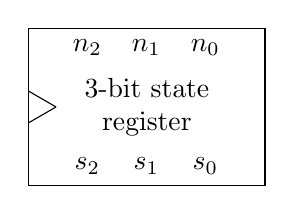
\begin{tikzpicture}[circuit logic US]
\draw (0,0) node (r) [shape=rectangle,draw,minimum height=2cm,minimum width=3cm,text width=2cm,align=center] {3-bit state register};
\draw (r) ++(left:11.54mm) -- ++($(left:3.46mm)+(down:2mm)$);
\draw (r) ++(left:11.54mm) -- ++($(left:3.46mm)+(up:2mm)$);
\draw (r.west) ++(up:7.5mm) ++(right:7.500000mm) node {$n_2$};
\draw (r.west) ++(down:7.5mm) ++(right:7.500000mm) node {$s_2$};
\draw (r.west) ++(up:7.5mm) ++(right:15.000000mm) node {$n_1$};
\draw (r.west) ++(down:7.5mm) ++(right:15.000000mm) node {$s_1$};
\draw (r.west) ++(up:7.5mm) ++(right:22.500000mm) node {$n_0$};
\draw (r.west) ++(down:7.5mm) ++(right:22.500000mm) node {$s_0$};
\end{tikzpicture}
\end{center}



\section{}
\begin{center}
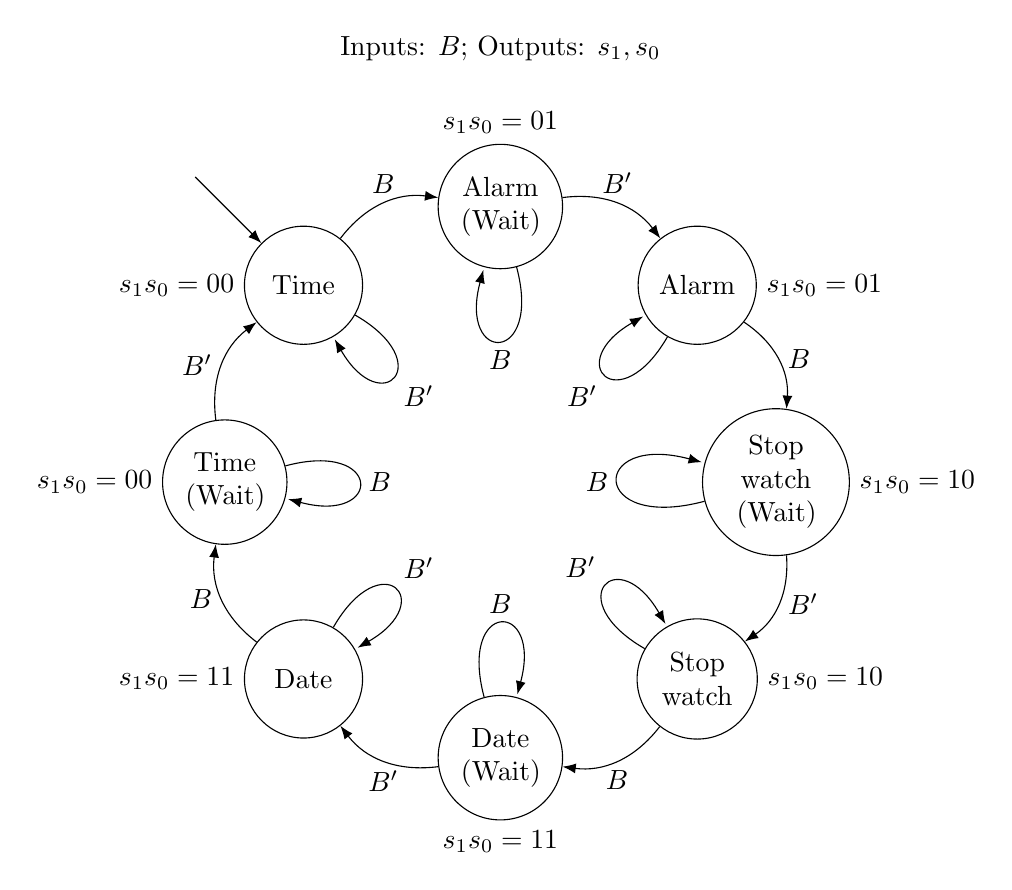
\begin{tikzpicture}[>/.tip={Latex}]
	\draw (0,5.5) node (io) {Inputs: $B$; Outputs: $s_1,s_0$};
	\draw (-2.5,2.5) node (C1) [draw,shape=circle,minimum size=1.5cm,text width=1cm,align=center] {Time};
	\node [left] at (C1.west) {$s_1s_0=00$};
	\draw (0,3.5) node (W2) [draw,shape=circle,minimum size=1.5cm,text width=1cm,align=center] {Alarm (Wait)};
	\node [above] at (W2.north) {$s_1s_0=01$};
	\draw (2.5,2.5) node (C2) [draw,shape=circle,minimum size=1.5cm,text width=1cm,align=center] {Alarm};
	\node [right] at (C2.east) {$s_1s_0=01$};
	\draw (3.5,0) node (W3) [draw,shape=circle,minimum size=1.5cm,text width=1cm,align=center] {Stop watch (Wait)};
	\node [right] at (W3.east) {$s_1s_0=10$};
	\draw (2.5,-2.5) node (C3) [draw,shape=circle,minimum size=1.5cm,text width=1cm,align=center] {Stop watch};
	\node [right] at (C3.east) {$s_1s_0=10$};
	\draw (0,-3.5) node (W4) [draw,shape=circle,minimum size=1.5cm,text width=1cm,align=center] {Date (Wait)};
	\node [below] at (W4.south) {$s_1s_0=11$};
	\draw (-2.5,-2.5) node (C4) [draw,shape=circle,minimum size=1.5cm,text width=1cm,align=center] {Date};
	\node [left] at (C4.west) {$s_1s_0=11$};
	\draw (-3.5,0) node (W1) [draw,shape=circle,minimum size=1.5cm,text width=1cm,align=center] {Time (Wait)};
	\node [left] at (W1.west) {$s_1s_0=00$};
	
	\draw[->] (C1) edge [bend left=30] node [above] {$B$} (W2);
	\draw[->] (W2) edge [bend left=30] node [above] {$B'$} (C2);
	\draw[->] (C2) edge [bend left=30] node [right] {$B$} (W3);
	\draw[->] (W3) edge [bend left=30] node [right] {$B'$} (C3);
	\draw[->] (C3) edge [bend left=30] node [below] {$B$} (W4);
	\draw[->] (W4) edge [bend left=30] node [below] {$B'$} (C4);
	\draw[->] (C4) edge [bend left=30] node [left] {$B$} (W1);
	\draw[->] (W1) edge [bend left=30] node [left] {$B'$} (C1);
	\draw[->] (C1) edge [in=300,out=330,loop] node [below right] {$B'$} ();
	\draw[->] (W2) edge [loop below] node [below] {$B$} ();
	\draw[->] (C2) edge [in=210,out=240,loop] node [below left] {$B'$} ();
	\draw[->] (W3) edge [loop left] node [left] {$B$} ();
	\draw[->] (C3) edge [in=120,out=150,loop] node [above left] {$B'$} ();
	\draw[->] (W4) edge [loop above] node [above] {$B$} ();
	\draw[->] (C4) edge [in=30,out=60,loop] node [above right] {$B'$} ();
	\draw[->] (W1) edge [loop right] node [right] {$B$} ();
	
	\draw (-4,4) node (init) {};
	\draw[->] (init) edge (C1);
\end{tikzpicture}
\end{center}

Encode the states ($s_2s_1s_0$): Time (Wait): 000, Time: 001, Alarm (Wait): 010, Alarm: 011, Stopwatch (wait): 100, Stopwatch: 101, Date (Wait): 110, Date (Wait): 111. \\

The truth table is 

\begin{center}
\begin{tabular}{cccc|ccccc}
$s_{2}$ & $s_{1}$ & $s_{0}$ & $B$ & $n_{2}$ & $n_{1}$ & $n_{0}$ & $s_1$ & $s_0$ \\
\hline
0 & 0 & 0 & 0 & 0 & 0 & 1 & 0 & 0 \\
0 & 0 & 0 & 1 & 0 & 0 & 0 & 0 & 0 \\
0 & 0 & 1 & 0 & 0 & 0 & 1 & 0 & 0 \\
0 & 0 & 1 & 1 & 0 & 1 & 0 & 0 & 0 \\
0 & 1 & 0 & 0 & 0 & 1 & 1 & 0 & 1 \\
0 & 1 & 0 & 1 & 0 & 1 & 0 & 0 & 1 \\
0 & 1 & 1 & 0 & 0 & 1 & 1 & 0 & 1 \\
0 & 1 & 1 & 1 & 1 & 0 & 0 & 0 & 1 \\
1 & 0 & 0 & 0 & 1 & 0 & 1 & 1 & 0 \\
1 & 0 & 0 & 1 & 1 & 0 & 0 & 1 & 0 \\
1 & 0 & 1 & 0 & 1 & 0 & 1 & 1 & 0 \\
1 & 0 & 1 & 1 & 1 & 1 & 0 & 1 & 0 \\
1 & 1 & 0 & 0 & 1 & 1 & 1 & 1 & 1 \\
1 & 1 & 0 & 1 & 1 & 1 & 0 & 1 & 1 \\
1 & 1 & 1 & 0 & 1 & 1 & 1 & 1 & 1 \\
1 & 1 & 1 & 1 & 0 & 0 & 0 & 1 & 1 \\
\end{tabular}
\end{center}

The euqations are 

$$n_{2}=s_{2}'s_{1}s_{0}B+s_{2}s_{1}'+s_{2}s_{0}'+s_{2}B'$$
$$n_{1}=s_{1}'s_{0}B+s_{1}s_{0}'+s_{1}B'$$
$$n_{0}=B'$$
$$s_1=s_{2}$$
$$s_0=s_{1}$$


The schematics is 

\begin{center}
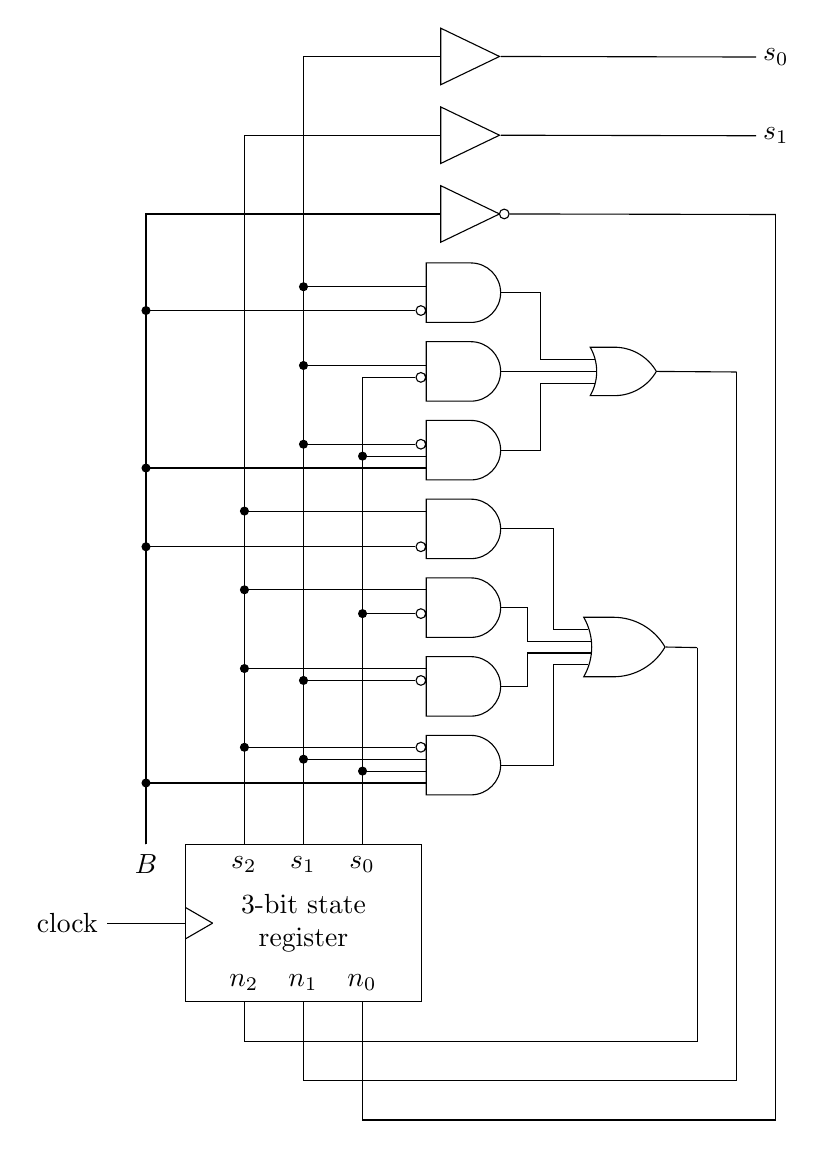
\begin{tikzpicture}[circuit logic US]
\draw (0,0) node (r) [shape=rectangle,draw,minimum height=2cm,minimum width=3cm,text width=2cm,align=center] {3-bit state register};
\draw (-3,0) node (clock) {clock};\draw (clock) -- (r.west);\draw (r) ++(left:11.54mm) -- ++($(left:3.46mm)+(down:2mm)$);
\draw (r) ++(left:11.54mm) -- ++($(left:3.46mm)+(up:2mm)$);
\draw (r.west) ++(up:7.5mm) ++(right:7.500000mm) node {$s_2$};
\draw (r.west) ++(down:7.5mm) ++(right:7.500000mm) node {$n_2$};
\draw (r.west) ++(up:7.5mm) ++(right:15.000000mm) node {$s_1$};
\draw (r.west) ++(down:7.5mm) ++(right:15.000000mm) node {$n_1$};
\draw (r.west) ++(up:7.5mm) ++(right:22.500000mm) node {$s_0$};
\draw (r.west) ++(down:7.5mm) ++(right:22.500000mm) node {$n_0$};
\draw (-2.000000,0.750000) node {$B$};
\draw (r.north) ++(up:1.000000cm) ++(right:2cm) node (and1) [and gate,inputs=innn] {};
\draw (-0.750000,1.000000) |- (and1.input 1) ;
\draw (0.000000,1.000000) |- (and1.input 2) ;
\draw (0.750000,1.000000) |- (and1.input 3) ;
\draw (-2.000000,1.000000) |- (and1.input 4) ;
\draw (r.north) ++(up:2.000000cm) ++(right:2cm) node (and2) [and gate,inputs=ninn] {};
\draw (-0.750000,1.000000) |- (and2.input 1) ;
\draw (0.000000,1.000000) |- (and2.input 2) ;
\draw (and1.input 1) ;
\pgfgetlastxy{\x}{\y};
\filldraw (-0.750000,\y) circle [radius=0.5mm];
\draw (and1.input 2) ;
\pgfgetlastxy{\x}{\y};
\filldraw (0.000000,\y) circle [radius=0.5mm];
\draw (r.north) ++(up:3.000000cm) ++(right:2cm) node (and3) [and gate,inputs=nnin] {};
\draw (-0.750000,1.000000) |- (and3.input 1) ;
\draw (0.750000,1.000000) |- (and3.input 3) ;
\draw (and2.input 1) ;
\pgfgetlastxy{\x}{\y};
\filldraw (-0.750000,\y) circle [radius=0.5mm];
\draw (and1.input 3) ;
\pgfgetlastxy{\x}{\y};
\filldraw (0.750000,\y) circle [radius=0.5mm];
\draw (r.north) ++(up:4.000000cm) ++(right:2cm) node (and4) [and gate,inputs=nnni] {};
\draw (-0.750000,1.000000) |- (and4.input 1) ;
\draw (-2.000000,1.000000) |- (and4.input 4) ;
\draw (and3.input 1) ;
\pgfgetlastxy{\x}{\y};
\filldraw (-0.750000,\y) circle [radius=0.5mm];
\draw (and1.input 4) ;
\pgfgetlastxy{\x}{\y};
\filldraw (-2.000000,\y) circle [radius=0.5mm];
\draw (r.north) ++(up:2.500000cm) ++(right:4cm) node (or1) [or gate,inputs=nnnn] {};
\draw (and1.output) -- ++(right:0.666667cm) |- (or1.input 4);
\draw (and2.output) -- ++(right:0.333333cm) |- (or1.input 3);
\draw (and3.output) -- ++(right:0.333333cm) |- (or1.input 2);
\draw (and4.output) -- ++(right:0.666667cm) |- (or1.input 1);
\draw (or1.output) -- (5.000000,3.500000);
\draw (5.000000,3.500000) -- (5.000000,-1.500000) -| (-0.750000,-1);
\draw (r.north) ++(up:5.000000cm) ++(right:2cm) node (and5) [and gate,inputs=ninn] {};
\draw (0.000000,1.000000) |- (and5.input 2) ;
\draw (0.750000,1.000000) |- (and5.input 3) ;
\draw (-2.000000,1.000000) |- (and5.input 4) ;
\draw (and2.input 2) ;
\pgfgetlastxy{\x}{\y};
\filldraw (0.000000,\y) circle [radius=0.5mm];
\draw (and3.input 3) ;
\pgfgetlastxy{\x}{\y};
\filldraw (0.750000,\y) circle [radius=0.5mm];
\draw (and4.input 4) ;
\pgfgetlastxy{\x}{\y};
\filldraw (-2.000000,\y) circle [radius=0.5mm];
\draw (r.north) ++(up:6.000000cm) ++(right:2cm) node (and6) [and gate,inputs=nnin] {};
\draw (0.000000,1.000000) |- (and6.input 2) ;
\draw (0.750000,1.000000) |- (and6.input 3) ;
\draw (and5.input 2) ;
\pgfgetlastxy{\x}{\y};
\filldraw (0.000000,\y) circle [radius=0.5mm];
\draw (and5.input 3) ;
\pgfgetlastxy{\x}{\y};
\filldraw (0.750000,\y) circle [radius=0.5mm];
\draw (r.north) ++(up:7.000000cm) ++(right:2cm) node (and7) [and gate,inputs=nnni] {};
\draw (0.000000,1.000000) |- (and7.input 2) ;
\draw (-2.000000,1.000000) |- (and7.input 4) ;
\draw (and6.input 2) ;
\pgfgetlastxy{\x}{\y};
\filldraw (0.000000,\y) circle [radius=0.5mm];
\draw (and5.input 4) ;
\pgfgetlastxy{\x}{\y};
\filldraw (-2.000000,\y) circle [radius=0.5mm];
\draw (r.north) ++(up:6.000000cm) ++(right:4cm) node (or2) [or gate,inputs=nnn] {};
\draw (and5.output) -- ++(right:0.500000cm) |- (or2.input 3);
\draw (and6.output) -- ++(right:0.000000cm) |- (or2.input 2);
\draw (and7.output) -- ++(right:0.500000cm) |- (or2.input 1);
\draw (or2.output) -- (5.500000,7.000000);
\draw (5.500000,7.000000) -- (5.500000,-2.000000) -| (0.000000,-1);
\draw (r.north) ++(up:8.000000cm) ++(right:2cm) node (and8) [not gate] {};
\draw (-2.000000,1.000000) |- (and8.input) ;
\draw (and7.input 4) ;
\pgfgetlastxy{\x}{\y};
\filldraw (-2.000000,\y) circle [radius=0.5mm];
\draw (and8.output) -- (6.000000,9.000000);
\draw (6.000000,9.000000) -- (6.000000,-2.500000) -| (0.750000,-1);
\draw (r.north) ++(up:9.000000cm) ++(right:2cm) node (and9) [buffer gate] {};
\draw (-0.750000,1.000000) |- (and9.input) ;
\draw (and4.input 1) ;
\pgfgetlastxy{\x}{\y};
\filldraw (-0.750000,\y) circle [radius=0.5mm];
\draw (and9.output) -- (5.750000,10.000000);
\draw (6,10.000000) node {$s_1$};
\draw (r.north) ++(up:10.000000cm) ++(right:2cm) node (and10) [buffer gate] {};
\draw (0.000000,1.000000) |- (and10.input) ;
\draw (and7.input 2) ;
\pgfgetlastxy{\x}{\y};
\filldraw (0.000000,\y) circle [radius=0.5mm];
\draw (and10.output) -- (5.750000,11.000000);
\draw (6,11.000000) node {$s_0$};
\end{tikzpicture}
\end{center}


\section{}
Same as Problem 7.

\end{document}
